% total_main.tex -- the eight section files inlined into one document, generated by
% scripts/flatten_paper.py.  Everything else (main.tex's preamble, style/, the .bib files, figure/) is
% unchanged and still required to build.  Edit the section files, not this one: regenerate it instead,
% or the next regeneration silently discards the edits.
%
\documentclass{article} % For LaTeX2e
% Target venue: ICLR 2027.  The kit under style/ is the 2025 one from the IGDM release; drop the
% 2027 .sty/.bst into style/ and change the two lines naming them.  Nothing else depends on the
% year.  Layout: this file + N_Section.tex are the manuscript, style/ is the venue kit, *.bib the
% bibliography, notes/ the prose companions that are NOT part of the build.
% 2026-09-05: the `times` option requests the ptm family, which has no TU (unicode) shapes under
% this engine, so every shape fell back to LM Roman regular and \textbf, \emph and \textsc were
% silently rendering as regular text -- paragraph headings and bold table rows included.  Forcing T1
% takes the legacy path, where ptm has its full set of shapes.
\usepackage[T1]{fontenc}
\usepackage{style/iclr2025_conference,times}

% Optional math commands from https://github.com/goodfeli/dlbook_notation.
\input{style/math_commands.tex}

\usepackage{hyperref}
\usepackage{url}

%%%%%%%%%%%%%%%%%%%%%%%%%%%%%% ADD PACKAGES %%%%%%%%%%%%%%%
\usepackage{subcaption}
\usepackage{amsmath}
\usepackage{amssymb}
\usepackage{amsthm}
\usepackage{cleveref}
\usepackage{booktabs}
\usepackage{multirow}
\newcommand{\ie}{\emph{i.e.}}

\usepackage{algorithm}
\usepackage{algorithmic}

\usepackage{array}
% FLOAT PLACEMENT (2026-09-05).  Every table was declared [t] and there are seven in the experiments
% section alone, so LaTeX ran out of top slots, deferred them, and dumped the queue at the end of the
% document -- tab:ladder and tab:controls were landing on page 25 of a 13-page body.  Widening the
% float parameters gives the placement algorithm room, and placeins puts a barrier at each section so
% a float can no longer cross out of the section that declares it.
\usepackage[section]{placeins}
\setcounter{topnumber}{3}
\setcounter{bottomnumber}{2}
\setcounter{totalnumber}{4}
\renewcommand{\topfraction}{0.92}
\renewcommand{\bottomfraction}{0.6}
\renewcommand{\textfraction}{0.06}
\renewcommand{\floatpagefraction}{0.7}
\usepackage{sidecap}
\usepackage{xcolor}   % [table] dropped: another package loads xcolor first, and we use no row colours

\usepackage{textgreek}
\usepackage{tikz}
\usepackage{wrapfig}

\setlength{\aboverulesep}{0.6pt}
\setlength{\belowrulesep}{1.5pt}

% Propositions and proofs were running into the surrounding prose and were hard to find when
% skimming.  amsthm's plain style (bold header, italic body) plus a little air around the environment
% is enough; an earlier version drew a rule down the left margin, which read as a quote block.
\theoremstyle{plain}
\newtheorem{proposition}{Proposition}
\newtheorem{corollary}{Corollary}
\makeatletter
\def\thm@space@setup{%
  \thm@preskip=1.4\parskip \@plus 3pt \@minus 1pt
  \thm@postskip=\thm@preskip}
\makeatother

% Run-in headings carry the structure of the experiments section, so give them room to be seen.
\makeatletter
\renewcommand{\paragraph}{\@startsection{paragraph}{4}{\z@}%
  {1.8ex \@plus 0.7ex \@minus .2ex}{-0.7em}%
  {\normalfont\normalsize\bfseries}}
\makeatother
\newcommand{\dg}{\textsuperscript{\dag}}
\newcommand{\ddg}{\textsuperscript{\ddag}}
%%%%%%%%%%%%%%%%%%%%%%%%%%%%%%%%%%%%%%%%%%%%%%%%%%%%%%%%%%%%

% Title framing note: an earlier version ended "...without a Robust Teacher", which invites the
% reading "so with a robust teacher you lose" -- and we would, since IGDM+AdaAD reaches
% 64.44/30.32 on this architecture from a WRN-28-10 teacher.  That is a ranking claim against a
% line this paper does not compete with.  The register here follows B-MTARD and ARREST, whose
% titles both name the goal ("Mitigating the Accuracy-Robustness Trade-off") and the mechanism,
% and claim nothing about what is unnecessary.
\title{Clean Feature Anchoring: Mitigating the Accuracy--Robustness\\
Trade-off by Self-Distilling a Naturally Trained Model}

\author{
Anonymous authors\\
Paper under double-blind review
}

\newcommand{\fix}{\marginpar{FIX}}
\newcommand{\new}{\marginpar{NEW}}

% \iclrfinalcopy   % uncomment only for the camera-ready; submissions must stay anonymous

\begin{document}

\maketitle

%% ============================================================================
%% 0_Abstract.tex
%% ============================================================================
\begin{abstract}
Adversarial training improves robustness but often sacrifices clean accuracy.
We mitigate this trade-off by first learning a clean self-teacher from natural
images and then preserving its knowledge during adversarial training.
We propose Clean Feature Anchoring (CFA), which anchors the student's
adversarial representation to the teacher's fixed clean representation while
retaining its classifier, without a label objective.
We connect this formulation to fixed clean-target regression and show that the
feature anchor jointly controls clean teacher fidelity and local feature
variation. We further introduce sensitivity-matched perturbation budgets to
account for example-dependent responses to adversarial perturbations.
On CIFAR-100 with ResNet-18, CFA achieves
\(64.82\mathbin{\pm}0.07\%\) clean and
\(28.04\mathbin{\pm}0.09\%\) AutoAttack accuracy, with consistent results
across CIFAR-10, Tiny-ImageNet, and WideResNet-34-10.
\end{abstract}

\section{Introduction}
\label{sec:intro}

Adversarial training improves robustness but often reduces clean accuracy
\citep{PGD,tsipras2018robustness,TRADES}. We ask whether robustness can be
learned while retaining more of the representation that supports strong clean
performance. Our approach separates these roles: we first train a clean
self-teacher only on natural images, then adversarially train a student while
preserving the teacher's clean knowledge. The teacher is not expected to be
robust; it provides the clean reference that the student seeks to retain.

This perspective differs from robust distillation methods that transfer
predictive distributions and balance them against label supervision
\citep{ard,rslad,adr,bmtard}. We instead use the clean teacher output as a
fixed target throughout the student's adversarial neighborhood. This leads to
\textbf{Clean Feature Anchoring (CFA)}: the student's adversarial feature is
matched to the teacher's clean feature while the inherited classifier remains
fixed. The adversarial-training stage therefore uses no label objective.

\begin{figure}[t]
  \centering
  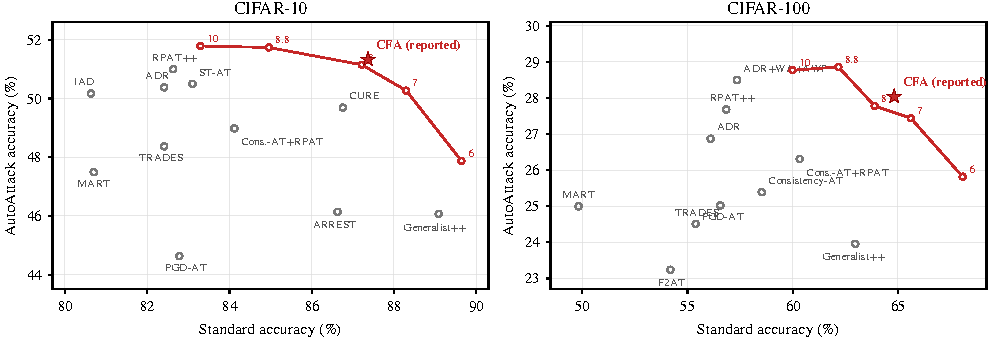
\includegraphics[width=\linewidth]{figure/frontier.pdf}
  \caption{Clean--AutoAttack trade-off on CIFAR-10 and CIFAR-100 with
  ResNet-18 at \(\epsilon=8/255\). Grey points are published results
  (\Cref{tab:published}); the CFA curve varies the training radius over
  100-epoch runs, and the star denotes the reported 150-epoch result.}
  \label{fig:frontier}
\end{figure}

Our analysis connects softened predictive supervision to direct regression on
a fixed clean target and characterizes what the feature anchor controls. It
also shows that teacher clean accuracy alone does not determine how much clean
performance transfers to the robust student. Finally, because the same pixel
radius can affect the anchor loss differently across examples, we redistribute
a fixed batch budget of attack radii according to local anchor sensitivity.
Thus the teacher specifies \emph{what} should be preserved, while sensitivity
matching determines \emph{where} that constraint is enforced most strongly.

Empirically, CFA improves the clean--robust trade-off across CIFAR-10,
CIFAR-100, Tiny-ImageNet, and WideResNet-34-10. On CIFAR-100 with ResNet-18,
it achieves \(64.82\mathbin{\pm}0.07\%\) clean and
\(28.04\mathbin{\pm}0.09\%\) AutoAttack accuracy across three runs.
Our contributions are: (i) a clean self-teacher framework that preserves clean
knowledge during label-free adversarial training; (ii) an analysis of fixed
clean-target transfer, including a joint fidelity--variation bound and evidence
that teacher accuracy alone does not characterize transferability; and
(iii) sensitivity-matched perturbation budgets that improve clean accuracy
without an observed loss of robustness in the final CIFAR-100 configuration.

\section{Related Work}
\label{sec:related}

\paragraph{Adversarial training and its targets.}
PGD adversarial training optimizes a model on worst-case inputs \citep{PGD}; TRADES separates clean
prediction from local consistency \citep{TRADES}, and MART reweights misclassified examples
\citep{MART}. Subsequent work improves generalization through label smoothing, consistency
regularization, weight averaging, and adversarial weight perturbation
\citep{pang2020bag,tack2022consistency,robustoverfit,2020_awp}. ADR replaces one-hot labels with
targets produced by an annealed momentum teacher \citep{adr}. These approaches motivate our study
of how the supervisory target affects the clean--robust trade-off.

\paragraph{Predictive targets in adversarial distillation.}
ARD transfers a robust teacher's predictions during adversarial training \citep{ard}. RSLAD emphasizes
robust soft labels \citep{rslad}, IAD discounts unreliable teacher guidance \citep{iad}, and AdaAD uses
the teacher in both adversarial-example generation and student optimization \citep{adaad}. IGDM adds
the teacher's local input geometry to logit-based distillation \citep{igdm}. These methods are designed
to inherit robustness from an adversarially trained teacher. Our target instead comes from a natural
teacher at the clean input and remains fixed during the student's inner maximization.

\paragraph{Guidance from naturally trained models.}
BGAT is the closest direct-regression precedent: it matches adversarial logits to a fixed natural
teacher's clean logits, and LBGAT extends this to a jointly trained natural branch \citep{lbgat}.
Our logit control confirms that this fixed-clean-target principle is not specific to features. CFA
uses the full clean representation with an inherited fixed classifier, and our analysis focuses on
what a single anchor controls, which teacher checkpoint supplies it, and how its neighborhood is
allocated. ARREST starts
from a naturally pretrained model and regularizes latent representations while retaining adversarial
cross-entropy and noisy replay \citep{arrest}. HAT uses a natural helper to label examples outside the
training ball \citep{hat}, and B-MTARD combines clean and robust teachers with adaptive temperature
and loss balancing \citep{bmtard}.

\paragraph{Sample-dependent perturbation budgets.}
IAAT and CAT adapt the training radius to sample difficulty, while MMA directly increases an
input-space margin \citep{iaat,cat,mma}. Our allocation has a different source: it redistributes a
fixed batch budget according to the input sensitivity of the loss being optimized. The comparison is
therefore not between adaptive and uniform radii alone, but between the signals used to assign the
same budget.

%% ============================================================================
%% 2_Analysis.tex
%% ============================================================================

\section{Analysis}
\label{sec:analysis}

We analyze how clean self-teacher knowledge should be transferred during
adversarial training. We first connect predictive distillation to fixed
clean-target regression, then characterize the feature anchor used by CFA,
and finally examine how teacher clean performance relates to transfer.

\subsection{From Predictive Distillation to a Fixed Clean Target}
\label{sec:fragile}
Let \(f=h\circ\Phi\), with feature map \(\Phi\) and linear classifier
\(h(z)=Wz+b\). Subscripts \(t\) and \(s\) denote the frozen clean teacher and
student. For clean \(x\) and \(x'\in B(x,\epsilon)\), shared-temperature KD uses
\begin{equation}
q_t^\tau(x)=\operatorname{softmax}(f_t(x)/\tau),\quad
p_s^\tau(x')=\operatorname{softmax}(f_s(x')/\tau),
\end{equation}
and \(\tau^2D_{\rm KL}(q_t^\tau\|p_s^\tau)\). For fixed logits, with
\(\bar f=f-C^{-1}\mathbf1\mathbf1^\top f\),
\begin{equation}
\lim_{\tau\to\infty}\tau^2D_{\rm KL}(q_t^\tau(x)\|p_s^\tau(x'))
=\frac{1}{2C}\|\bar f_t(x)-\bar f_s(x')\|_2^2.
\label{eqn:kd_limit}
\end{equation}
Thus high-temperature predictive distillation approaches centered-logit
regression. CFA applies the same fixed-clean-target principle in feature space:
\begin{equation}
\mathcal L_{\rm anchor}(x)=\max_{x'\in B(x,\epsilon)}
\|\Phi_s(x')-\Phi_t(x)\|_2^2.
\label{eqn:anchor_percell}
\end{equation}
Feature matching is a design choice rather than a consequence of
\Cref{eqn:kd_limit}; empirically, direct logit and feature regression reach
similar operating points (\Cref{fig:targetcomparison,tab:regression_stack}).

\begin{figure}[t]
  \centering
  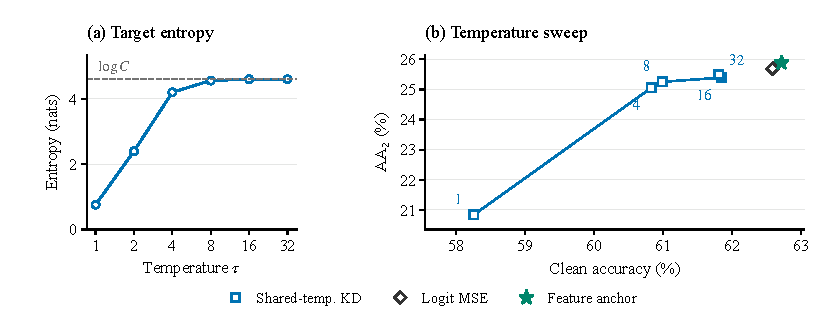
\includegraphics[width=\linewidth]{figure/analysis_targets.pdf}
  \caption{Target comparison on CIFAR-100 (ResNet-18). (a) Entropy of the
  clean teacher target as the shared temperature increases. (b) Clean accuracy
  and AA under shared-temperature KD, direct logit regression, and feature
  regression. Exact values are in \Cref{tab:targetcomparison_values}.}
  \label{fig:targetcomparison}
\end{figure}

A key distinction is where the teacher is evaluated. A perturbed teacher
feature can inherit the vulnerability of the natural teacher: replacing the
fixed target \(\Phi_t(x)\) with \(\Phi_t(x_{\rm adv})\) yields
\(76.11\%\) clean accuracy but \(0.00\%\) AA, whereas the fixed clean target
reaches \(61.33/26.19\) clean/AA under the same 50-epoch control
(\Cref{tab:teacherread}). This supports using the natural teacher as a clean
reference rather than asking the student to reproduce its perturbed response.

\subsection{What the Anchor Controls}
\label{sec:decomp}
For \(B=B(x,\epsilon)\), define
\begin{equation}
L=\max_{x'\in B}\|\Phi_s(x')-\Phi_t(x)\|_2,\quad
F=\|\Phi_s(x)-\Phi_t(x)\|_2,\quad
O=\max_{x',x''\in B}\|\Phi_s(x')-\Phi_s(x'')\|_2.
\end{equation}
\begin{proposition}[Fixed-anchor decomposition]\label{prop:decomp}
For every \(x\) and \(\epsilon\ge0\), \(L\le F+O\le3L\).
\end{proposition}
The result follows from the triangle inequality; the proof and scope are in
\Cref{app:anchor_scope}. Hence \(L\le\delta\) implies \(F\le\delta\) and
\(O\le2\delta\): one fixed anchor controls both clean teacher fidelity and
local feature variation, without requiring the teacher itself to be robust.
The same argument applies to any norm-based fixed target, including logits,
and does not establish that feature coordinates are inherently superior.

\subsection{Teacher Clean Performance and Transferability}
\label{sec:teacher_transfer}
Higher teacher clean accuracy need not produce a student with higher clean
accuracy after adversarial training. Along one CIFAR-100 teacher trajectory,
teacher clean accuracy rises from \(75.81\%\) to \(78.32\%\), while student
clean accuracy falls from \(64.28\%\) to \(62.24\%\) and AA rises from
\(24.38\%\) to \(25.80\%\) (\Cref{fig:teacherladder}). An independent
trajectory shows the same overall pattern (\Cref{tab:teacherladder_seed1}).
Moreover, label-smoothed and mixup teachers differing by only \(0.14\) points
in clean accuracy produce students differing by \(4.18\) clean points, with
nearly identical AA (\Cref{tab:matchedteacher}). Teacher clean accuracy is
therefore an incomplete descriptor of transferability. We fix the 200-epoch
teacher as a reference for the remaining experiments.

\section{Method}
\label{sec:method}
The analysis motivates two components: a fixed clean representation target and
a sample-dependent perturbation budget.

\subsection{Clean Feature Anchoring}
\label{sec:anchor}
Let \(\Phi_t,h_t\) denote the frozen clean self-teacher. The student inherits
\(\Phi_s\leftarrow\Phi_t\) and \(h_s=h_t\), after which only \(\Phi_s\) is
optimized. For each clean example,
\begin{equation}
 x_{\rm adv}=\arg\max_{x'\in B(x,\epsilon)}
 \|\Phi_s(x')-\Phi_t(x)\|_2^2,\qquad
 \mathcal L_{\rm CFA}=\mathbb E_x\|\Phi_s(x_{\rm adv})-\Phi_t(x)\|_2^2.
\label{eqn:anchor}
\end{equation}
We approximate the inner maximization with randomly initialized PGD. No label
loss is used in this stage, and inference uses \(h_t\circ\Phi_s\). The full
procedure is given in \Cref{alg:cfa}.

\subsection{Sensitivity-Matched \(\epsilon\)}
\label{sec:angeps}
A uniform pixel radius can induce different changes in the anchor loss across
examples. For
\(\ell_{\rm anc}(x';x_i)=\|\Phi_s(x')-\Phi_t(x_i)\|_2^2\), first-order
movement in an \(\ell_\infty\) ball satisfies
\begin{equation}
\max_{\|\delta\|_\infty\le e}\langle\nabla_{x'}\ell_{\rm anc},\delta\rangle
=e\|\nabla_{x'}\ell_{\rm anc}\|_1.
\label{eqn:firstorder}
\end{equation}
Motivated by this relation, let \(g_i>0\) be a local sensitivity score. We
allocate
\begin{equation}
\epsilon_i=N\epsilon\frac{g_i^{-p}}{\sum_{j=1}^N g_j^{-p}},
\label{eqn:angeps_ideal}
\end{equation}
so \(\sum_i\epsilon_i=N\epsilon\). Thus the method redistributes, rather than
increases, the batch perturbation budget; \(p=0\) recovers a uniform radius.
Implementation details, clipping, and the sensitivity-norm control are reported
in \Cref{app:box}.

\section{Experiments}
\label{sec:exp}

We evaluate whether CFA improves the clean--robust trade-off, generalizes beyond the default setting, and whether its two defining components account for the gain.

\subsection{Experimental Settings}
We evaluate CIFAR-10, CIFAR-100 \citep{krizhevsky2009learning}, and Tiny-ImageNet-200 \citep{le2015tiny}, using ResNet-18 by default and WideResNet-34-10 for model-scale transfer. Unless stated otherwise, the clean self-teacher is trained on natural images for 200 epochs and frozen; the student inherits its backbone and fixed classifier. Main CIFAR runs use 150 epochs, AdamW, a one-cycle schedule, PGD-10, \(\epsilon_{\rm train}=8/255\), sensitivity matching (\(p=1\)), WA, and AWP. We report clean and AutoAttack (AA) accuracy at \(8/255\), their arithmetic mean (Avg), and harmonic mean (NRR). Full settings and attack diagnostics are in \Cref{app:repro,app:gradmask}.

\subsection{Main Results}
\begin{table}[!htbp]
  \centering
  \footnotesize
  \setlength{\tabcolsep}{3.2pt}
  \caption{
  ResNet-18 results under \(\ell_\infty\) perturbations with
  \(\epsilon=8/255\). All values are measured in our framework.
  \emph{T.} denotes the teacher assumed by each method: none (--),
  a natural model (nat.), or the method's own weight average (self).
  The CIFAR-100 CFA row reports the mean of three student seeds;
  all other rows are individual runs.
  }
  \label{tab:main}
  \begin{tabular}{llrrrrrrrr}
    \toprule
    & & \multicolumn{4}{c}{CIFAR-10}
      & \multicolumn{4}{c}{CIFAR-100} \\
    \cmidrule(lr){3-6}\cmidrule(lr){7-10}
    Method & T. & Clean & AA & Avg & NRR
           & Clean & AA & Avg & NRR \\
    \midrule
    PGD-AT & -- & 84.54 & 43.57 & 64.06 & 57.50
                 & 57.36 & 20.34 & 38.85 & 30.03 \\
    TRADES & -- & 81.71 & 49.16 & 65.44 & 61.39
                 & 55.28 & 23.55 & 39.42 & 33.03 \\
    MART   & -- & 80.41 & 45.56 & 62.99 & 58.16
                 & 53.86 & 22.72 & 38.29 & 31.96 \\
    \midrule
    ARD & nat. & 84.58 & 43.75 & 64.16 & 57.67
               & 57.61 & 20.24 & 38.93 & 29.96 \\
    RSLAD & nat. & 85.15 & 42.91 & 64.03 & 57.06
                 & 59.68 & 21.30 & 40.49 & 31.40 \\
    AdaAD & nat. & 85.39 & 46.22 & 65.81 & 59.98
                 & 59.79 & 23.19 & 41.49 & 33.42 \\
    AdaAD + IGDM & nat. & 85.01 & 45.50 & 65.26 & 59.27
                        & 48.25 & 19.48 & 33.87 & 27.75 \\
    LBGAT & nat. & -- & -- & -- & --
                 & 56.46 & 26.02 & 41.24 & 35.62 \\
    ARREST & nat. & 85.06 & 46.42 & 65.74 & 60.06
                  & \textbf{66.97} & 22.78 & 44.88 & 34.00 \\
    \midrule
    HAT & nat. & 84.59 & 48.81 & 66.70 & 61.90
               & 60.67 & 24.45 & 42.56 & 34.85 \\
    ADR & self & 83.36 & 49.72 & 66.54 & 62.29
               & 59.93 & 27.20 & 43.57 & 37.42 \\
    RPAT++ & -- & 82.41 & 50.75 & 66.58 & 62.82
                  & 55.93 & 27.36 & 41.64 & 36.74 \\
    \midrule
    \textbf{CFA (ours)}
      & nat.
      & \textbf{87.37} & \textbf{51.33}
      & \textbf{69.35} & \textbf{64.67}
      & \textbf{64.82} & \textbf{28.04}
      & \textbf{46.43} & \textbf{39.15} \\
    \bottomrule
  \end{tabular}
\end{table}

On CIFAR-100, CFA reaches \(64.82\%\) clean and \(28.04\%\) AA (NRR
\(39.15\)); relative to ADR, the closest baseline in NRR, this is
\(+4.89\) clean, \(+0.84\) AA, and \(+1.73\) NRR points. On CIFAR-10, CFA
reaches \(87.37/51.33\) clean/AA and an NRR of \(64.67\), exceeding the
closest baseline NRR by \(1.85\) points (\Cref{tab:main}).

\subsection{Generalization}
\begin{table}[!htbp]
  \centering
  \footnotesize
  \setlength{\tabcolsep}{3.2pt}
  \caption{
  Results on Tiny-ImageNet-200 with ResNet-18 and CIFAR-10 with
  WideResNet-34-10, measured in our framework.
  }
  \label{tab:scale}
  \begin{tabular}{llrrrrrrrr}
    \toprule
    & & \multicolumn{4}{c}{Tiny-ImageNet, ResNet-18}
      & \multicolumn{4}{c}{CIFAR-10, WRN-34-10} \\
    \cmidrule(lr){3-6}\cmidrule(lr){7-10}
    Method & T. & Clean & AA & Avg & NRR
           & Clean & AA & Avg & NRR \\
    \midrule
    PGD-AT & -- & 49.72 & 14.45 & 32.09 & 22.39
                 & 86.00 & 45.71 & 65.86 & 59.69 \\
    TRADES & -- & 46.98 & 15.95 & 31.46 & 23.83
                 & 85.13 & 48.99 & 67.06 & 62.19 \\
    MART & -- & 46.01 & 16.90 & 31.46 & 24.73
               & 85.29 & 47.06 & 66.18 & 60.65 \\
    \midrule
    ARD & nat. & 49.74 & 14.48 & 32.11 & 22.43
               & 86.35 & 45.52 & 65.94 & 59.61 \\
    RSLAD & nat. & 51.26 & 17.02 & 34.14 & 25.56
                 & 86.41 & 45.80 & 66.10 & 59.87 \\
    AdaAD & nat. & 51.59 & 16.79 & 34.19 & 25.33
                 & 86.80 & 46.84 & 66.82 & 60.85 \\
    LBGAT & nat. & 51.04 & 18.47 & 34.75 & 27.13
                 & 81.56 & 51.79 & 66.68 & 63.35 \\
    ARREST & nat. & \textbf{59.38} & 16.06 & 37.72 & 25.28
                  & 87.54 & 48.83 & 68.19 & 62.69 \\
    HAT & nat. & 52.57 & 17.28 & 34.93 & 26.01
               & 87.15 & 53.21 & 70.18 & 66.07 \\
    ADR & self & 47.66 & \textbf{20.85} & 34.25 & 29.01
               & 88.64 & 52.34 & 70.49 & 65.82 \\
    \midrule
    \textbf{CFA (ours)}
      & nat.
      & 55.16 & 20.54 & \textbf{37.85} & \textbf{29.93}
      & \textbf{88.67} & \textbf{55.29}
      & \textbf{71.98} & \textbf{68.11} \\
    \bottomrule
  \end{tabular}
\end{table}

CFA also transfers across data and model scale. On Tiny-ImageNet it reaches
\(55.16/20.54\) clean/AA, and on CIFAR-10 with WideResNet-34-10 it reaches
\(88.67/55.29\). On CIFAR-100 with the same architecture, CFA obtains
\(65.04/30.14\), compared with ADR at \(64.50/29.04\)
(\Cref{tab:wrn100}).

\subsection{Ablation and Component Analysis}
\label{sec:components}
\paragraph{Clean feature anchoring.}
\begin{table}[!htbp]
  \centering
  \small
  \setlength{\tabcolsep}{5pt}
  \caption{
  Objective control on CIFAR-100 with ResNet-18, 100 epochs, no weight
  averaging or AWP, \(p=0\), and
  \(\epsilon_{\mathrm{train}}=8.8/255\).
  }
  \label{tab:controls}
  \begin{tabular}{lrrr}
    \toprule
    Objective & Clean & AA & NRR \\
    \midrule
    Anchor
      & \textbf{61.29} & \textbf{25.36} & \textbf{35.88} \\
    Label cross-entropy, same recipe
      & 54.60 & 19.45 & 28.68 \\
    Label cross-entropy, own recipe
      & 56.66 & 20.91 & 30.55 \\
    \bottomrule
  \end{tabular}
\end{table}

Without WA, AWP, or sensitivity matching, the anchor exceeds label
cross-entropy by \(6.69\) clean and \(5.91\) AA points under the same recipe;
it remains ahead when cross-entropy uses its own optimizer and schedule
(\Cref{tab:controls}). Together with the clean-versus-perturbed teacher-target
control in \Cref{sec:fragile}, this isolates the fixed clean anchor from the
surrounding training stack.

\paragraph{Sensitivity-matched radius allocation.}
\begin{table}[!htbp]
  \centering
  \small
  \setlength{\tabcolsep}{5pt}
  \caption{
  Clean-target regression in the final CIFAR-100 recipe
  (ResNet-18, 150 epochs, \(\epsilon_{\mathrm{train}}=8/255\)).
  Feature rows report mean \(\pm\) sample standard deviation over three
  student seeds and differ only in \(p\); logit regression is one run at
  \(p=1\).
  }
  \label{tab:finalallocation}
  \begin{tabular}{lrrr}
    \toprule
    Target and radius & Clean & AA & NRR \\
    \midrule
    Features, uniform (\(p=0\))
      & \(62.63\pm0.22\)
      & \(28.01\pm0.20\)
      & \(38.71\pm0.21\) \\
    Features, sensitivity-matched (\(p=1\))
      & \(\mathbf{64.82\pm0.07}\)
      & \(\mathbf{28.04\pm0.09}\)
      & \(\mathbf{39.15\pm0.09}\) \\
    Logits, sensitivity-matched (\(p=1\))
      & 64.49 & 27.85 & 38.90 \\
    \bottomrule
  \end{tabular}
\end{table}

Across three paired runs, sensitivity matching improves clean accuracy by
\(2.19\pm0.20\) points while AA changes by only \(0.03\pm0.23\) points. The
clean gain appears in every seed, whereas the AA difference is within
run-to-run variation. Direct logit regression remains close to feature
regression, consistent with the fixed-target interpretation.

\paragraph{Does the allocation signal matter?}
\begin{table}[!htbp]
  \centering
  \small
  \setlength{\tabcolsep}{4.5pt}
  \caption{
  Radius-allocation signals under the same mean radius on CIFAR-100 with
  ResNet-18, trained for 100 epochs with WA and AWP.
  \(\mathrm{sd}(w)\) measures multiplier dispersion.
  }
  \label{tab:allocation}
  \begin{tabular}{lrrrr}
    \toprule
    Allocation & \(\mathrm{sd}(w)\) & Clean & AA & NRR \\
    \midrule
    Uniform
      & 0 & 60.42 & 28.42 & 38.66 \\
    Sensitivity
      & 0.32 & \textbf{62.17} & \textbf{28.86} & \textbf{39.42} \\
    Same multipliers, difficulty order
      & 0.32 & 60.90 & 28.06 & 38.42 \\
    Difficulty magnitude
      & 0.39 & 61.27 & 28.12 & 38.55 \\
    Logit margin
      & 0.42 & 61.07 & 27.79 & 38.20 \\
    \bottomrule
  \end{tabular}
\end{table}

Reassigning the same sensitivity-derived radius multipliers by sample
difficulty reduces AA by \(0.80\) points and NRR by \(1.00\) point, despite
preserving the radius distribution. Thus heterogeneous radii alone do not
explain the gain. Additional recipe, radius, and WA/AWP controls are reported
in \Cref{tab:baselinestack,tab:radius,tab:stackboth,tab:ladder}.

\section{Conclusion}
CFA addresses the clean--robust trade-off by learning clean knowledge first
and preserving it during adversarial training. A fixed clean target provides
a simple alternative to softened predictive supervision, while the feature
realization jointly controls teacher fidelity and local feature variation.
Sensitivity-matched radii further improve retained clean accuracy without an
observed AA loss in the final CIFAR-100 setting. The results across datasets,
architectures, and controls support clean self-teaching as a practical route
to robust training without an adversarial teacher or label objective during
the robust stage.


% The appendix is kept in a separate file so the nine-page main body can be
% edited independently while preserving cross-references in the full build.
\input{appendix_revised.tex}

\bibliography{AT,cfa}
\bibliographystyle{style/iclr2025_conference}
\end{document}
